% Provenance (never printed): see sources/outline_sources.md and sources/book1/BRIEFS.md (g5/01).
% Powers of two appear only as doubling (the mathematics books bring powers in grade 8).
\chapter{Bits and Bytes: Counting in Binary}\label{ch:g5:bits-and-bytes}

It is getting dark, and Sami and Noor stand at the two ends of the playground,
each with a torch. With one torch, Sami can send only two messages: light on
means ``come here'', light off means ``stay there''. So he takes a second torch.
Now there are four ways to hold them: both off, only the left one on, only the
right one on, both on. Four messages! With a third torch they would have eight.
A \omterm{def:g1:what-is-a-computer:computer}{computer} does exactly the same thing, with billions of tiny switches.

\begin{omfigure}
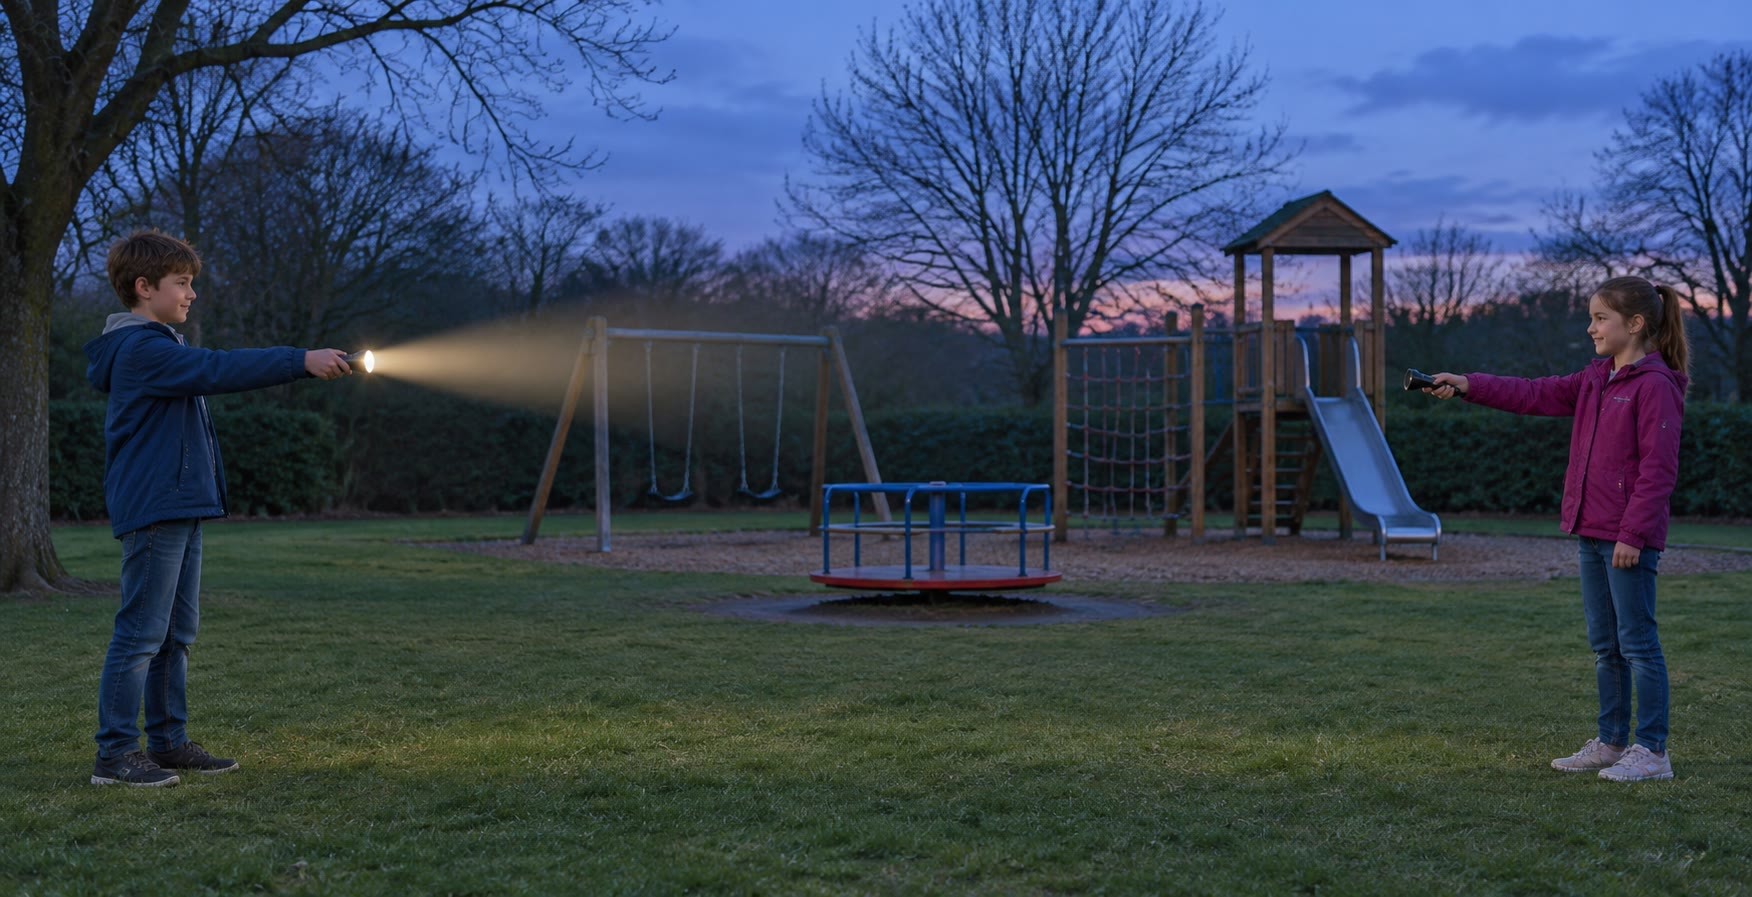
\includegraphics[width=0.62\linewidth]{images/book1/ai/g5-bits-and-bytes-torches.jpg}

{\small Signalling across the playground: each torch is on or off.}
\end{omfigure}

\begin{recall}
Sizes in a \omterm{def:g1:what-is-a-computer:computer}{computer} are counted in \omterm{def:g4:memory-and-storage:byte}{bytes}; one \omterm{def:g4:memory-and-storage:byte}{byte} holds one letter of plain
text. The \omterm{def:g3:inside-the-computer:storage}{storage} keeps information without electricity
(\cref{ch:g4:memory-and-storage}).
\end{recall}

\section{Two states are enough}

Inside a \omterm{def:g1:what-is-a-computer:computer}{computer}, every tiny part that holds information can be in one of two
states only. A switch is on or off. A tiny area of a \omterm{def:g4:memory-and-storage:hard-disk}{hard disk} is magnetised
one way or the other. A cell of \omterm{def:g4:memory-and-storage:flash}{flash memory} holds an electric charge or does
not. Two states are easy to make, easy to tell apart, and hard to mix up.

\begin{definition}[Bit]\label{def:g5:bits-and-bytes:bit}
A \emph{bit}\index{bit} is the smallest piece of information: one choice
between two states. We write the two states 0 and 1.
\end{definition}

\begin{omfigure}
\begin{tikzpicture}[x=1cm, y=1cm, font=\footnotesize]
  \node[anchor=west, font=\small\bfseries] at (-0.2,1.9) {hard disk surface};
  \foreach \b [count=\i] in {1,0,1,1,0,0,1,0} {
    \draw[black!50, fill=black!6] (0.9*\i-0.9,0.6) rectangle ++(0.9,0.8);
    \ifnum\b=1 \draw[-{Stealth[length=2mm]}, thick, ocRed!80!black] (0.9*\i-0.75,1.0) -- ++(0.6,0);
    \else \draw[-{Stealth[length=2mm]}, thick, ocBlue!80!black] (0.9*\i-0.15,1.0) -- ++(-0.6,0); \fi
    \node at (0.9*\i-0.45,0.3) {\b};
  }
  \begin{scope}[shift={(8.2,0)}]
  \node[anchor=west, font=\small\bfseries] at (-0.2,1.9) {flash memory cells};
  \foreach \b [count=\i] in {1,0,1,1,0,0,1,0} {
    \draw[black!50, fill=black!6, rounded corners=1pt] (0.6*\i-0.6,0.6) rectangle ++(0.5,0.8);
    \ifnum\b=1 \foreach \dy in {0.8,1.0,1.2} \fill[ocRed!80!black] (0.6*\i-0.35,\dy) circle (0.06); \fi
    \node at (0.6*\i-0.35,0.3) {\b};
  }
  \end{scope}
\end{tikzpicture}

{\small The same eight \omterm{def:g5:bits-and-bytes:bit}{bits}, 10110010, kept in two ways. On a \omterm{def:g4:memory-and-storage:hard-disk}{hard disk}, each
tiny area is magnetised to the right or to the left; in \omterm{def:g4:memory-and-storage:flash}{flash memory}, each cell
holds a charge (the dots) or not. The drawing is much simplified.}
\label{fig:g5:bits-and-bytes:states}
\end{omfigure}

\section{Counting with two digits}

How can numbers be written with only 0 and 1? Take five cards. The card on the
right has 1 dot, the next one 2 dots, then 4, then 8, then 16: each card has
twice as many dots as the card on its right. Each card is either face up, and
its dots count, or face down, and it counts nothing.

\begin{omfigure}
\begin{tikzpicture}[x=1cm, y=1cm, font=\small,
    dcard/.style={draw=black!70, rounded corners=3pt, minimum width=1.9cm, minimum height=2.5cm}]
  \foreach \v/\b [count=\i] in {16/0, 8/1, 4/1, 2/0, 1/1} {
    \ifnum\b=1 \node[dcard, fill=white] (c\i) at (2.3*\i,0) {};
    \else \node[dcard, fill=ocBlue!45] (c\i) at (2.3*\i,0) {}; \fi
    \node[font=\footnotesize] at (2.3*\i,1.6) {\v};
    \node[font=\Large\bfseries] at (2.3*\i,-1.65) {\b};
  }
  % dots on the face-up cards (8, 4, 1)
  \foreach \x in {-0.5,-0.17,0.17,0.5} \foreach \y in {0.3,-0.3} \fill (2.3*2+\x,\y) circle (0.1);
  \foreach \x/\y in {-0.3/0.3, 0.3/0.3, -0.3/-0.3, 0.3/-0.3} \fill (2.3*3+\x,\y) circle (0.1);
  \fill (2.3*5,0) circle (0.1);
  \node[anchor=west, align=left] at (12.4,0) {$8 + 4 + 1$\\$= 13$};
\end{tikzpicture}

{\small The number 13 with five cards: 8, 4 and 1 face up, 16 and 2 face down
(the blue backs). Reading the cards from left to right, face up as 1 and face
down as 0, gives 01101.}
\label{fig:g5:bits-and-bytes:cards}
\end{omfigure}

With the five cards, any number from 0 (all face down) to 31 (all face up,
$16 + 8 + 4 + 2 + 1$) can be shown, each in exactly one way.

\begin{definition}[Binary]\label{def:g5:bits-and-bytes:binary}
Writing a number in \emph{binary}\index{binary} is writing it with the
digits 0 and 1 only, where each place is worth twice the place on its right:
1, 2, 4, 8, 16, and so on, from the right. A number written this way is a
\emph{binary number}\index{binary number}.
\end{definition}

\begin{method}[Writing a number in binary]\label{met:g5:bits-and-bytes:to-binary}
Start with the largest card that is not more than the number: turn it face up
and take its value away from the number. Go on with the next cards to the
right: turn a card face up if its value is not more than what is left, and
take it away. When nothing is left, read the cards: 1 for face up, 0 for face
down.
\end{method}

\begin{example}[Writing 22 and reading 10011]\label{ex:g5:bits-and-bytes:22}
For 22: 16 fits, 6 is left; 8 does not fit; 4 fits, 2 is left; 2 fits, 0 is
left; 1 does not fit. So 22 is 10110 in \omterm{def:g5:bits-and-bytes:binary}{binary}. To read 10011, add the values
of the places that hold a 1: $16 + 2 + 1 = 19$.
\end{example}

Counting in \omterm{def:g5:bits-and-bytes:binary}{binary} is like counting with ordinary numbers, but each place is
full after 1 instead of after 9: 0, 1, 10, 11, 100, 101, 110, 111, 1000\dots

\section{A byte is eight bits}

The \omterm{def:g4:memory-and-storage:byte}{byte} of the chapter on \omterm{def:g3:inside-the-computer:memory}{memory} and \omterm{def:g3:inside-the-computer:storage}{storage} is made of \omterm{def:g5:bits-and-bytes:bit}{bits}: a \omterm{def:g4:memory-and-storage:byte}{byte} is eight \omterm{def:g5:bits-and-bytes:bit}{bits}. With eight
cards, worth 128, 64, 32, 16, 8, 4, 2 and 1, any number from 0 to 255 can be
shown: $128 + 64 + 32 + 16 + 8 + 4 + 2 + 1 = 255$. So one \omterm{def:g4:memory-and-storage:byte}{byte} can hold any
whole number from 0 to 255.

\begin{omfigure}
\begin{tikzpicture}[x=1cm, y=1cm, font=\small]
  \foreach \v/\b [count=\i] in {128/0, 64/0, 32/1, 16/0, 8/1, 4/1, 2/0, 1/1} {
    \node[font=\footnotesize] at (1.3*\i,1.0) {\v};
    \ifnum\b=1
      \fill[ocYellow!80] (1.3*\i,0) circle (0.42);
      \foreach \a in {0,45,...,315} \draw[ocYellow!80!black, thick] (1.3*\i,0) ++(\a:0.5) -- ++(\a:0.16);
    \else \fill[black!20] (1.3*\i,0) circle (0.42); \fi
    \draw[black!60] (1.3*\i,0) circle (0.42);
    \node[font=\large\bfseries] at (1.3*\i,-0.85) {\b};
  }
  \node[anchor=west, align=left] at (11.2,0) {$32 + 8 + 4 + 1$\\$= 45$};
\end{tikzpicture}

{\small A \omterm{def:g4:memory-and-storage:byte}{byte} as eight lamps: on for 1, off for 0. Above each lamp, the value
of its place. The \omterm{def:g4:memory-and-storage:byte}{byte} 00101101 is the number 45.}
\label{fig:g5:bits-and-bytes:byte}
\end{omfigure}

\section{Each extra bit doubles the patterns}

How many different patterns can a few \omterm{def:g5:bits-and-bytes:bit}{bits} make? One \omterm{def:g5:bits-and-bytes:bit}{bit} has two patterns: 0
and 1. Two \omterm{def:g5:bits-and-bytes:bit}{bits} have four: 00, 01, 10, 11. For three \omterm{def:g5:bits-and-bytes:bit}{bits}, take each of these
four and add a 0 or a 1 at the end: that makes twice as many, eight patterns.

\begin{omfigure}
\begin{forest}
  for tree={font=\footnotesize\ttfamily, draw=black!50, rounded corners=1.5pt, inner sep=2pt,
    l sep=6mm, s sep=1.5mm, edge={black!50}, fill=white},
  [start, font=\footnotesize\sffamily, fill=black!8
    [0 [00 [000] [001]] [01 [010] [011]]]
    [1 [10 [100] [101]] [11 [110] [111]]]]
\end{forest}

\medskip
{\footnotesize\sffamily 1 \omterm{def:g5:bits-and-bytes:bit}{bit}: 2 patterns \quad 2 \omterm{def:g5:bits-and-bytes:bit}{bits}: 4 patterns \quad 3 \omterm{def:g5:bits-and-bytes:bit}{bits}: 8 patterns}

{\small The tree of choices. Each new \omterm{def:g5:bits-and-bytes:bit}{bit} splits every pattern in two, so the
number of patterns doubles.}
\label{fig:g5:bits-and-bytes:tree}
\end{omfigure}

\begin{proposition}[Doubling]\label{prop:g5:bits-and-bytes:doubling}
Each extra \omterm{def:g5:bits-and-bytes:bit}{bit} doubles the number of different patterns: 2 patterns with one
\omterm{def:g5:bits-and-bytes:bit}{bit}, 4 with two, 8 with three, 16 with four, and so on. With eight \omterm{def:g5:bits-and-bytes:bit}{bits}, one
\omterm{def:g4:memory-and-storage:byte}{byte}, there are 256 patterns: the numbers 0 to 255.
\end{proposition}

\begin{proof}
Each pattern of $n$ \omterm{def:g5:bits-and-bytes:bit}{bits} gives two patterns of $n + 1$ \omterm{def:g5:bits-and-bytes:bit}{bits}, one ending in 0 and one
ending in 1. Every pattern of $n + 1$ \omterm{def:g5:bits-and-bytes:bit}{bits} comes from exactly one pattern of $n$
\omterm{def:g5:bits-and-bytes:bit}{bits}: the one left when its last \omterm{def:g5:bits-and-bytes:bit}{bit} is taken away. So there are twice as
many patterns of $n + 1$ \omterm{def:g5:bits-and-bytes:bit}{bits}.
\end{proof}

Doubling grows very fast. Keep doubling from 2, eight times: 2, 4, 8, 16, 32,
64, 128, 256. Twenty more doublings would take us past 268 million.

\section{Exercises}

\begin{exercise}[$\star$]\label{exo:g5:bits-and-bytes:1}
Write 5, 9 and 20 in \omterm{def:g5:bits-and-bytes:binary}{binary} with five cards.
\end{exercise}

\begin{exercise}[$\star$]\label{exo:g5:bits-and-bytes:2}
Which number is written 11010 in \omterm{def:g5:bits-and-bytes:binary}{binary}?
\end{exercise}

\begin{exercise}[$\star$]\label{exo:g5:bits-and-bytes:3}
What is the largest number that can be shown with four cards? With five? With
eight?
\end{exercise}

\begin{exercise}[$\star$]\label{exo:g5:bits-and-bytes:4}
How many different patterns can 4 \omterm{def:g5:bits-and-bytes:bit}{bits} make? Find it by doubling.
\end{exercise}

\begin{exercise}[$\star$]\label{exo:g5:bits-and-bytes:5}
Count from 0 to 7 in \omterm{def:g5:bits-and-bytes:binary}{binary}, using three digits each time.
\end{exercise}

\begin{exercise}[$\star$]\label{exo:g5:bits-and-bytes:6}
How many \omterm{def:g5:bits-and-bytes:bit}{bits} are needed to write 40 in \omterm{def:g5:bits-and-bytes:binary}{binary}? Try with the cards.
\end{exercise}

\begin{exercise}[$\star$]\label{exo:g5:bits-and-bytes:7}
These eight lamps show a \omterm{def:g4:memory-and-storage:byte}{byte} (yellow is on). Which number is it?

\begin{center}
\begin{tikzpicture}[x=0.75cm, y=0.75cm]
  \foreach \b [count=\i] in {1,0,0,1,0,0,1,1} {
    \ifnum\b=1 \fill[ocYellow!80] (\i,0) circle (0.3); \else \fill[black!20] (\i,0) circle (0.3); \fi
    \draw[black!60] (\i,0) circle (0.3);
  }
\end{tikzpicture}
\end{center}
\end{exercise}

\begin{exercise}[$\star$]\label{exo:g5:bits-and-bytes:8}
Give three things, in a \omterm{def:g1:what-is-a-computer:computer}{computer} or elsewhere, that have exactly two states.
\end{exercise}

\begin{exercise}[$\star\star$]\label{exo:g5:bits-and-bytes:9}
The cards show 0111. Add 1: which cards turn over? What is the new number in
\omterm{def:g5:bits-and-bytes:binary}{binary}, and in ordinary numbers?
\end{exercise}

\begin{exercise}[$\star\star$]\label{exo:g5:bits-and-bytes:10}
The teacher wants to give each of the 50 pupils of the school's two classes a
different code of 6 \omterm{def:g5:bits-and-bytes:bit}{bits}. Are there enough codes?
\end{exercise}

\begin{exercise}[$\star\star$]\label{exo:g5:bits-and-bytes:11}
Why must the value of each card be twice the value of the card on its right?
What would go wrong with cards worth 1, 2, 3, 4 and 5?
\end{exercise}
